%!TEX root = ../../../ECP-ST-CAR.tex 

\subsubsection{\stid{5.10} ExaWorks} \label{subsubsect:exaworks}

% ECP ST Project Overviews: A significant portion of this report includes 2-page synopses of each
% ECP ST project (Section 4), including a project overview, key challenges, solution strategy, recent progress and next steps

\paragraph{Overview} Exascale computing capacity reinforces the need for workflows and also creates
a slew of new workflow challenges. Most notably, the increasing scale and
hardware heterogeneity demands higher level programming environments, such as
workflows, to enable a broad range of scientists, students, and developers to
describe complex computational procedures and manage their execution at
enormous scales in intuitive and productive ways. Further, in addition to the
changing system architectures, application patterns are also changing: no
longer is research conducted with a single invocation of a lone executable,
instead it typically requires orchestration of many applications and scripts,
executed at various scales across many different resource types, and often
reliant on machine learning algorithms for guidance. As a result, exascale
Workflow Management Systems (WMSs) will need to support high performance
execution of significant numbers of short-duration tasks (e.g., inference
tasks), efficient scheduling of tasks with varying resource (e.g., single
core, multiple nodes, and accelerators) and time-sensitive (e.g., coupling
data analysis with simulations) constraints, and flexible coordination and
communication patterns between many concurrent jobs and/or tasks.


\paragraph{Key Challenges}
Emerging exascale workflows pose significant challenges to the creation of
portable, repeatable, and performant workflows. These challenges are both
technical and non-technical. On the technical side, WMSs are currently
incapable of supporting the needs of heterogeneous co-scheduled and
high-throughput workflows, as well as enabling communication between fine
grain tasks in dynamic workflows. On the non-technical side, the myriad WMSs
that exist, lack of reusable WMS components, and the lack of clear user
guidance when selecting a WMS has resulted in a disjoint workflows community
that tends toward building ad hoc or bespoke solutions rather than adopting
and extending existing solutions.

Specific challenges include: 
\begin{enumerate}
    \item Workflows community: the workflows, applications, and facility communities are disjoint. Efforts are needed to bring these groups together to agree on common workflow components and interfaces, and to work together to develop, integrate, and support these components.
    \item Scheduling: exascale workflows must manage the efficient execution of diverse
    tasks (e.g., in runtime, resource requirements, single/multi-node) with complex interdependencies on increasingly heterogeneous resources. 
    \item Scale and performance: emerging workflows feature huge ensembles of short-running jobs, which can create millions or even billions of tasks that need to be rapidly scheduled and executed.
    \item Coordination and communication: workflows depend on coordination between the workflow and the tasks within the workflow, a need that requires efficient exchange of data following various communication patterns.
    \item Fault tolerance: the enormous number of computing elements and workflow tasks increases the likelihood of encountering faults within a workflow both at the system level and also from the millions of concurrent tasks. 
    \item Portability: most WMSs are tested on a handful of systems and the frequency by which system hardware and software change makes it impossible to guarantee that a workflow will work on even the same system in the future.
\end{enumerate}

\paragraph{Solution Strategy}
The ExaWorks project will lay the foundation for an inherently
\textit{new approach} to workflows: establishing the ExaWorks toolkit (see
Figure~\ref{fig:arch}) by assembling shared components from existing workflow
projects. The ExaWorks toolkit will provide a robust, well-tested, documented,
and scalable set of components that can be combined to enable diverse teams to
produce scalable and portable workflows for a wide range of exascale
applications. Importantly, the project will not create a new workflow system
nor does it aim not to replace the many workflow solutions already deployed
and used by scientists, but rather it will provide well engineered and
scalable components which can be leveraged by new and existing workflows.


\begin{wrapfigure}[15]{r}{0.5\textwidth}
\begin{center}
    \includegraphics[width=0.5\textwidth]{projects/2.3.5-Ecosystem/2.3.5.10-ExaWorks/exaworks.png}
    %\includegraphics[width=0.4\textwidth]{exaworks.png}
  \end{center}
  \caption{ExaWorks Toolkit\label{fig:arch}}
\end{wrapfigure} 

The goals of the initial phase of the project are to instantiate the ExaWorks community, 
bringing together workflow tool developers, ECP applications, and DOE compute facility representatives.  Specifically, it will:
\begin{enumerate}
    \item Engage the facilities to survey the state of workflow tools and capabilities and ways in which ExaWorks can enhance their capabilities;
    \item Establish an advisory board composed of representatives of DOE compute facilities, ECP applications, and workflow tools, to guide and advise ExaWorks;
    \item Survey ECP applications teams to identify the tools currently being used and to identify common challenges and needs;
    \item Assemble a functional design working group to develop a community-centered draft function design; and
    \item Collaborate with ECP applications to develop a proof-of-concept integration using a shared functional component as defined by the draft design, in an ECP application.
\end{enumerate}

\paragraph{Recent Progress}
In this first period of the project we have
assembled our advisory committee, 
started a functional design working group, and distributed a workflows
survey to the ECP community. The results of this survey are helping
to prioritize in-person interviews as well as informing the 
functional design process and helping to identify initial ExaWorks components. 
Our team have started prototyping efforts to explore 
component-based approaches in existing workflow systems. Specifically, 
we have developed prototype Balsam and RADICAL-Pilot executors for Parsl
which enable Parsl workflows to leverage the resource management 
capabilities of these external systems.


\paragraph{Next Steps}
The remainder of this initial effort focuses on four important areas. 
First, continuing to grow the ExaWorks community by engaging with ECP 
applications, facilities, and WMS teams. 
Second, working with these partners and stakeholders to produce a draft
functional design document that outlines ExaWorks components
and potential interfaces to these components. 
Third, we will produce a report, derived from interviews from 
the broad ECP community that outlines ECP workflows needs, challenges, 
and potential solutions. 
Finally, we will demonstrate the technical feasibility of the 
ExaWorks approach via application of preliminary components to
at least one ECP application. 
